% Chapter Template

\chapter{Descripteurs d'Images \&  Mesures de Similarité} % Main chapter title

\label{Chapter2} % Change X to a consecutive number; for referencing this chapter elsewhere, use \ref{ChapterX}

%----------------------------------------------------------------------------------------
%	SECTION 1
%----------------------------------------------------------------------------------------

\section{Introduction}
Aujourd’hui avec le développement des systèmes multimédias, nous utilisons de plus en plus le contenu visuel comme support de communication dans différents domaines. En effet l’image et la vidéo numérique sont partie intégrante de tels systèmes par la densité et la richesse de leur contenu. La même image peut présenter plusieurs significations à différents niveaux : analyse, description, reconnaissance et interprétation. Dans notre domaine, le premier but de n’importe quel système de recherche d’images est de fournir des résultats totalement satisfaits pour l'utilisateur, ce qui nécessite d’utiliser les meilleures méthodes d’extraction de caractéristiques (Descripteurs) et les représenter d’une manière réduite afin d’atteindre un temps de réponse acceptable pour un système de recherche d'images. L'information obtenue dans cette étape d'extraction est une sorte de résumé des images de la base. La transformation est généralement gourmande en temps de calcul.\\

Dans ce chapitre, nous présentons les différents descripteurs utilisés dans les systèmes de recherche d'image par contenu et ensuite les mesures de similarité entre les images après la définition de leurs vecteurs descripteurs (signatures ou attributs).




%----------------------------------------------------------------------------------------
%	SECTION 2
%----------------------------------------------------------------------------------------

\section{Descripteurs d'image}
Le CBIR diffère de la recherche d’information textuelle essentiellement par le fait que les bases de données d’images sont non-structurées, les images numériques n’étant que des matrices d’intensités de pixels, sans signification inhérente les unes par rapport aux autres. Donc avant même de commencer à faire des hypothèses sur le contenu de l’image, une des questions clé dans tout type de traitement d’image est l’extraction de l'information utile à partir de ces matrices de pixels.\\

Une grande partie du choix des descripteurs employés et des techniques associées à leur extraction permet d’avoir des systèmes de recherche d’images performants et robustes.
\paragraph{Définition:}
Un descripteur est défini comme la connaissance utilisée pour caractériser l'information contenue dans les images
[Nguy09]. 

De nombreux descripteurs sont développés et utilisés dans les systèmes de recherche pour décrire les images. Ceux-ci peuvent être différenciés selon deux niveaux :

\begin{table}[H]
	\begin{center}
		\caption{Classification des descripteurs.}
		\begin{tabular}{|l|l|}
			\hline
			\multicolumn{1}{|c|}{\textbf{Les descripteurs bas niveau}}                                                                                       & \multicolumn{1}{c|}{\textbf{Les descripteurs haut niveau}}                                                                                                                                                                                                   \\ \hline
			\begin{tabular}[c]{@{}l@{}}Décrivent le contenu bas niveau de \\ l'image, principalement en termes \\ de couleur, texture et forme.\end{tabular} & \begin{tabular}[c]{@{}l@{}}Décrivent le contenu sémantique \\ de l'image, et sont principalement\\ des mots clès fournis par l'utilisateur \\ lors de l'indexation, car l'extraction\\  automatique est un problème non \\ résolu actuellement.\end{tabular} \\ \hline
		\end{tabular}
		
	\end{center}
\end{table}

Les études que nous allons réaliser portent principalement sur des descripteurs bas-niveau, par la mise en place des descripteurs couleur, texture et forme.\\  

L'extraction de descripteurs peut avoir deux méthodes différentes, les descripteurs globaux qui sont extraits à partir de l’image entière et les descripteurs locaux qui sont calculés d'une partie de l'image. Les descripteurs calculés sur toute l’image permettent de minimiser le temps de calculs, la taille de données nécessaires ainsi que le coût. Au contraire, les descripteurs locaux sont bien adaptés aux images manipulées, mais l’utilisation de cette méthode reste longue et coûteuse.

 
%----------------------------------------------------------------------------------------
%	SUBSECTION 1
%----------------------------------------------------------------------------------------
\subsection{Les descripteur de la couleur}
La couleur est l’information visuelle la plus utilisée dans les systèmes de recherche par le contenu. Ces valeurs tridimensionnelles font que son potentiel discriminatoire soit supérieur à la valeur en niveaux de gris des images. Mais la caractérisation de la couleur dans une image est une opération extrêmement complexe. En effet, cette donnée varie considérablement avec l’orientation des surfaces, le point de vue de la caméra et l’illumination (positions et longueur d'onde des sources lumineuses). En outre, la perception de la couleur par l'être humain est un processus complexe et subjectif [Ouhda19].

\begin{figure}[H]
	\label{fig:imageRVB}
	\centering
	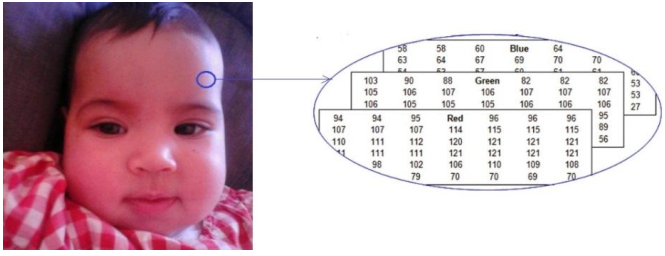
\includegraphics[width=0.65\textwidth]{Figures/imageRVB} % Include the image .png
	
	\caption{Image couleur dans l’espace RVB.}
	
\end{figure}

La couleur est devenue un attribut largement utilisé dans les systèmes opérationnels de recherche d'images par le contenu. Elle facilite l'identification et l'extraction d'un objet dans une scène [Zavi01]. Il semble que son efficacité à ce stade soit liée au fait que l'être humain peut distinguer des milliers de couleurs et seulement 24 niveaux de gris [Gonz02].\\

Généralement, la couleur est représentée par un espace colorimétrique de trois composantes. De nombreux travaux ont vu le jour quant à l’utilisation de la couleur pour la recherche d’images par le contenu. L’approche la plus courante dans la littérature est l’histogramme couleur.

\subsubsection{L'histogramme}
La plus grande majorité des systèmes de recherche d'images par le contenu se base sur la description des couleurs composant les images. L'histogramme des couleurs exprime la distribution statistique de celles-ci dans l'image.

Ce type d'histogramme est calculé typiquement sur un espace caractéristique quantifié. Chaque valeur de caractère dans l'histogramme représente donc un rang de couleur dans la palette. 

L'histogramme a été introduit pour la première fois en RIC (Recherche d'iformation par le contenu) par [Swain91], depuis il est très utilisé à cause de sa simplicité de calcul, son invariance aux changements d'échelle et aux transformations géométriques.\\

\begin{figure}[H]
	\label{fig:hist}
	\centering
	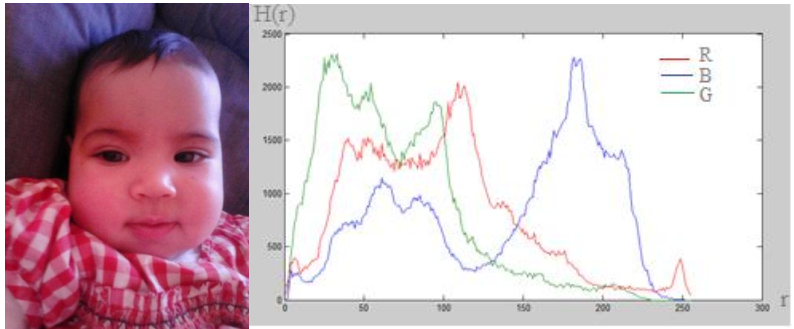
\includegraphics[width=0.65\textwidth]{Figures/hist} % Include the image .png
	\caption{Exemple d’histogramme d’une image couleur.}
\end{figure}

Les inconvénients majeurs de l'histogramme sont:
\begin{itemize}
	\item La perte de toute information spatiale dont la texture ou la forme. Par exemple un histogramme d'un tapis rouge peut être très proche de celui d'une porte rouge ou d'une voiture rouge.
	
	\item Ils sont de grandes tailles, donc par conséquent il est difficile de créer une indexation rapide et efficace en les utilisant tels qu'ils sont. 
	
	\item Ils sont sensibles à de petits changements de luminosité, ce qui est problématique pour comparer des images similaires, mais acquises dans des conditions différentes. 
	
	\item Ils sont inutilisables pour la comparaison partielle des images (objet particulier dans une image), puisque calculés globalement sur toute l’image.
	
\end{itemize}

\begin{figure}[H]
	\label{fig:samehist}
	\centering
	
\includegraphics[width=0.45\textwidth]{Figures/sameHist} % Include the image .png
	\caption{Deux images différentes de même histogramme.}
\end{figure}

Des méthodes alternatives ont été proposées pour augmenter l'efficacité de l'histogramme. Nous citons quelques-unes : 
\begin{itemize}
	\item les moments de la couleur [Stricker94], 
	\item les constantes de couleur [Flickner95],
	\item la signature couleur [Kender98], 
	\item les blobs [Chang97] et le vecteur cohérent de couleur [Pass97].
\end{itemize}


%----------------------------------------------------------------------------------------
%	subsubSECTION 2
%----------------------------------------------------------------------------------------
\subsubsection{Les moments de couleur}
Les moments de couleur on été utilisés dans plusieurs systèmes de recherche d’images par le contenu tel que QBIC (IBM's Query By Image Content). Mathématiquement, cette approche consiste à calculer l’espérance, l’équivalent d’une moyenne pondérée de tous les couleurs, puis la variance et les moments d’ordre 3 pour chaque composante couleur par les formules suivantes :

\begin{equation}
	\mu_i = \frac{1}{N} \sum_{j=1}^{N} p_{ij}
\end{equation}

\begin{equation}
	\sigma_i = \sqrt{\frac{1}{N} \sum_{j=1}^{N} (p_{ij}-\mu_i)^2}
\end{equation}

\begin{equation}
	s_i = \sqrt[3]{\frac{1}{N} \sum_{j=1}^{N} (p_{ij}-\mu_i)^3}
\end{equation}

Où $p_{ij}$ représente la valeur du pixel, $N$ représente le nombre total des pixels dans cette image.\\


La méthode d'histogramme utilise la distribution complète de la couleur. On doit stocker de nombreuses données. Au contraire, Les moments de couleur est une représentation compacte comparée aux autres descripteurs de couleur. Car seulement 9 valeurs (3 pour chaque composante chromatique) sont utilisées pour représenter le contenu d'une image. Dans [Stricker95], les auteurs ont prouvé que les méthodes des moments statistiques utilisées marchent plus vite et donnent des résultats meilleurs que les méthodes d’histogrammes.\\


%
%\subsubsection{Conclusion}
%L'information relative aux couleurs est particulièrement importante dans la caractérisation d’une image. Plusieurs études ont été menées pour trouver un critère de choix des descripteurs de couleurs pour l'indexation des images, mais aucune n'est pas suffisamment efficace. Ceci peut s’expliquer par le manque de subjectivité de cette information, les descripteurs couleur ne suffisent pas à indexer efficacement une image, ni à la chercher.
%
%Dans plusieurs domaines d’application, l’utilisation de descripteurs résumant l’information globale d’images couleurs n’offre pas toujours des résultats satisfaisants. Globalement, l’histogramme couleur reste le descripteur le plus utilisé vue qu'il garde un fort pouvoir de description. Bien qu’il ne contienne qu’une information partielle en raison de l’absence d’indication sur les caractéristiques spatiales.

%----------------------------------------------------------------------------------------
%	SUBSECTION 2
%----------------------------------------------------------------------------------------
\subsection{Descripteur de la texture}
Au même titre que la couleur, la texture est un  attribut visuel largement utilisé dans la recherche d’images par le contenu. Elle est également importante pour caractériser les motifs présents dans l’image. Elle permet de combler un vide que la couleur est incapable de faire, notamment lorsque les distributions de couleurs sont très proches. L'identification de la texture est une partie importante du système visuel humain, c'est un arrangement spatial de pixels, habituellement dans des modèles visuels homogènes que la couleur ne décrivent suffisamment. La modélisation et la description des textures est un problème difficile. La texture est une caractéristique intuitive facile à reconnaître mais difficile à définir.

%-------------------------------------
%            SUBSUBSECTION
%-----------------------------------------
\subsubsection{Définitions}

D'après [Bimbo99], une définition formelle de la texture est quasiment impossible. De nombreuses définitions ont été proposées, mais aucune ne convient parfaitement aux différents types de textures rencontrées. Dans une définition couramment citée [Policarpo98], la texture est présentée comme une structure disposant de certaines propriétés spatiales homogènes et invariantes par translation. Cette définition stipule que la texture donne la même impression à l'observateur quelle que soit la position spatiale de la fenêtre à travers laquelle il observe cette texture. Par contre l'échelle d’observation doit être précisée. On peut le faire par exemple en précisant la taille de la fenêtre d’observation.\\

En générale, la notion de texture est liée à trois concepts principaux:
\begin{enumerate}
	\item Un certain ordre local qui se répète dans une région de taille assez grande,
	
	\item Cet ordre est défini par un arrangement structuré de ses constituants élémentaires,
	
	\item Ces constituants élémentaires représentent des entités uniformes qui se caractérisent par des dimensions semblables dans toute la région considérée.\\ 
	
\end{enumerate}

\begin{figure}[H]
	\label{fig:textures}
	\centering
	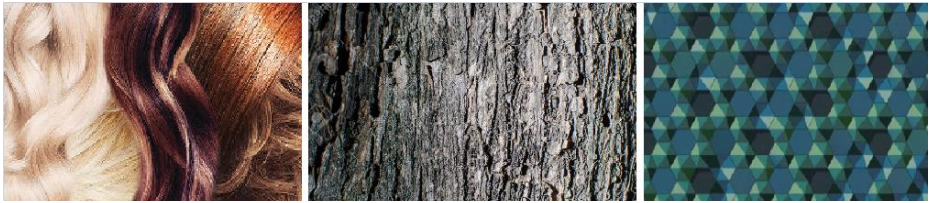
\includegraphics[width=0.65\textwidth]{Figures/textures} % Include the image .png
	\caption{Exemple des textures différentes.}
\end{figure}

\begin{description}
	\item[Définition 1:] 	
	D'une manière générale, la texture dans une image peut être définie comme un arrangement spatial de couleurs ou d'intensités dans une région de cette image [Linda01]. Elles peuvent consister en un placement structuré d’éléments mais peuvent aussi n’avoir aucun élément répétitif.
\end{description}

\begin{description}
	\item[Définition 2:] 	
	La texture peut être vue comme un ensemble de pixels (niveaux de gris) spatialement agencés selon un certain nombre de relations spatiales, ainsi créant une région homogène.
\end{description}

%-------------------------------------
%            SUBSUBSECTION
%-----------------------------------------
\subsubsection{Classifications de textures}
Il existe un grand nombre de textures. On peut les séparer en deux classes:
\begin{itemize}
	\item \textbf{Les textures structurées (macrotextures):} constituées par la répétition d’une primitive à intervalle régulier. On peut différencier dans cette classe les textures parfaitement périodiques (carrelage, damier, ...etc.), les textures dont la primitives subit des déformations ou des changements d'orientation (mur de briques, grains de café, ...etc.).
	
	\item \textbf{Les textures aléatoires (microtextures):} se distinguent en général par un aspect plus fin (sable, herbe, ...etc.). Contrairement aux textures de type structurel, les textures aléatoires ne comportent ni primitive isolable, ni fréquence de répétition. On ne peut donc pas extraire de ces textures une primitive qui se répète dans l’image mais plutôt un vecteur de paramètres statistiques homogènes à chaque texture.
\end{itemize}

Dans tous les cas, il est nécessaire d'extraire l'un ou plusieurs paramètres caractéristiques de cette texture. Nous désignerons ces paramètres sous le terme d’attributs texturaux (textural features).\\

Certains de ces paramètres correspondent à une propriété visuelle de la texture (comme la directionnalité ou la rugosité). D'autres correspondent à des propriétés purement mathématiques auxquelles il est difficile d'associer une qualification perceptive.
Un recensement ainsi qu'une classification des termes de description des textures employés par les principaux auteurs pourront être trouvés dans [Rao93] et [Lohse93].\\

De ces définitions et classifications, les recherches sur la modélisation des textures se sont portées sur la caractérisation de ces relations spatiales [Gueg07]. Quatre types d’approches se distinguent [Tuce98] [Zhan02] : 
les approches statistiques, les méthodes géométriques, les méthodes à base de modèles probabilistes et les méthodes fréquentielles. Ainsi, les attributs texturaux peuvent être obtenus à partir d’un ensemble assez vaste de différentes théories mathématiques, nous citons notamment :

\begin{table}[H]
	\begin{center}
		\caption{Classification des méthodes d’extraction de texture.}
		\begin{tabular}{ll}
			\hline
			\multicolumn{1}{|c|}{\textit{\textbf{Approche}}} & \multicolumn{1}{c|}{\textit{\textbf{Descripteur}}}  \\                             \hline 
			
			\multicolumn{1}{|c|}{\textbf{Statistiques}}      & \multicolumn{1}{l|}{\begin{tabular}[c]{@{}l@{}}- Matrice de longueur de plage\\ - Matrice de co-occurrence\\ - Méthode de différence de niveaux de gris\\ - Caractéristique de Tamura\\ - Méthode de dépendance spatiale des niveaux de gris\end{tabular}}  \\ \hline
			
			\multicolumn{1}{|c|}{\textbf{Fréquentielles}}    & \multicolumn{1}{l|}{\begin{tabular}[c]{@{}l@{}}- Transformée de Fourier discrète\\ - Filtre de Gabor\\ - Les ondelettes\end{tabular}}  \\ \hline
			
			\multicolumn{1}{|c|}{\textbf{\makecell{Méthodes à base\\ de modèle}}}    & \multicolumn{1}{l|}{\begin{tabular}[c]{@{}l@{}}- Décomposition de Wold\\ - Modèles Fractals\\ - Modèles AR (Autoregressive Models)\end{tabular}}  	\\ \hline
			
		\end{tabular}
		
	\end{center}
\end{table}


\subsubsection{Les matrices de co-occurrences (Mesures de Haralick)}
 En 1973, Haralick a proposé une méthode en se basant sur la matrice de co-occurrence de niveaux de gris [Haralick73], elle est probablement une méthode classiques et la plus célèbre pour l'analyser de la texture.
 
 La texture d'une image peut être interprétée comme la régularité d'apparition de couples de niveaux de gris selon une distance (pas $k=1, 2, 3, ...etc$) donnée dans l’image. La matrice de co-occurrences contient les fréquences spatiales relatives d’apparition des niveaux
 de gris selon quatre directions: $\theta = 0◦$,  $\theta =  \frac{\pi}{4} = 45◦$,  $\theta =  \frac{\pi}{2} = 90◦$,  $\theta =  3 \times \frac{\pi}{4} = 135◦$. Une matrice de co-occurrences est définie au moyen d’une relation entre deux pixels .\\

\begin{description}
	\item[Définition] La matrice de coocurrence $P_{d,\theta}=(P_{d,\theta}(i, j))_{1\leq i,j \leq Ng}$ est une matrice carrée de taille $Ng \times Ng$. Avec:
	\begin{itemize}
		\item Ng étant le nombre de niveaux de gris de l'image (256x256). Les indices de la matrice de co-occurrences sont
		donc les niveaux de gris de la texture étudiée.
		\item On réduit souvent a des tailles 8x8, 16x16 ou 32x32.
		\item L’élément $P_{d,\theta}(i, j)$de la matrice de cooccurrence définit la fréquence d'apparition des couples de niveaux de gris $i$ et $j$ pour les couples de pixels séparés par une distance $d$ dans la direction $\theta$.
		
		\begin{equation}
			P_{d,\theta}(i, j) = \sum_{x,y} 1_{ [I(x, y) = i \space \&\& \space  I(i + d, j + d) = v ]}
		\end{equation}
		Où: $ 1_{ [bool]} = 1 $ si $ bool = vrai $ sinon 0.
	\end{itemize} 
Pour obtenir de véritables fréquences relatives, il faut normaliser les éléments de la matrice en les divisant par le nombre total de paires de points élémentaires séparés par la distance d dans la direction dans toute l’image.
\end{description}

Alors on peut calculer plusieurs matrices, pour chaque distance (pas) et direction, mais avec un temps de calcul de ces matrices est assez long.

Soit l’image I définie par:

\begin{figure}[H]
	\label{fig:cooc}
	\centering
	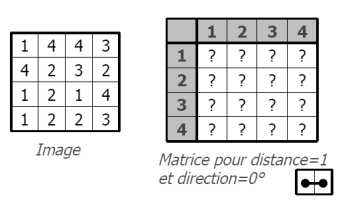
\includegraphics[width=0.65\textwidth]{Figures/cooc} % Include the image .png
	\caption{Matrice de co-occurrence.}
\end{figure}

On parcours l'image et pour chaque couple de pixels formé avec la distance et la direction données, on incrémente la matrice des co-occurrences de 1. Alors la matrice de co-occurrence (non normalisée) est:

\begin{figure}[H]
	\label{fig:cooc_nn}
	\centering
	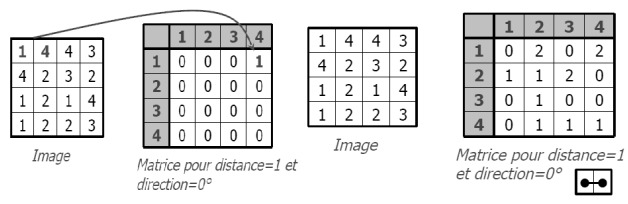
\includegraphics[width=0.8\textwidth]{Figures/cooc_non_norm} % Include the image .png
	\caption{Principe d'une atrice de co-occurrence:
	(a) et (c): image originale, (b): debut de calcul et (d): matrice de co-occurrence finale}
\end{figure}

Le 2 de la matrice de co-occurrence (ligne 1 et colonne 4) signifie que l’on trouve deux fois un pixel de valeur 1 de distance 1 et de direction
0 d’un pixel de valeur 4.\\


A partir de cette matrice de co-occurrence, il est possible de définir plusieurs descripteurs (Mesures de Haralick), tels que ceux répertoriés dans cette table:

\begin{table}[H]
	\centering
	\caption{Mesures de Haralick}
	\begin{tabular}{|c|c|c|}
		
		\hline
		\textbf{ Mesure} & \textbf{  Formulation} \\
		\hline
		Uniformité/Energie & \makecell{$E = \sum_{i=0}^{n}\sum_{j=0}^{n} P_{d,\theta}(i, j) $ }    \\
		\hline
		Entropie & \makecell{$En = -\sum_{i=0}^{n}\sum_{j=0}^{n} P_{d,\theta}(i, j) \log_2 (P_{d,\theta}(i, j)) $}    \\
		\hline
		Contraste & \makecell{$ C = \sum_{i=0}^{n}\sum_{j=0}^{n} P_{d,\theta}(i, j) (i-j)^2 $} \\
		\hline
	Moment inverse de différence & \makecell{$ M = \frac{1}{1+(i-j)^2} \sum_{i=0}^{n}\sum_{j=0}^{n} P_{d,\theta}(i, j)  $}\\
	     \hline
	\end{tabular}

\end{table}
 
 
\subsubsection{Transformée en ondelettes}
 Le terme " ondelette " en anglais (wavelet) a été utilisé pour la première fois en 1984 par J. Morlet et A. Grossmann pour résoudre des problèmes de traitement des signaux pour la prospection pétrolière. La transformée en ondelettes est à la base de nombreuses analyses de texture, telles que les filtres de Haar [Ganesan07].
 
 Une ondelette est une fonction à la base de la décomposition en ondelettes, décomposition similaire à la transformée de Fourier à court terme. La transformée en ondelettes consiste à décomposer un signal par une cascade de filtres pour générer une famille d'ondelettes appelées les ondelettes filles, obtenues par la translation et la dilatation d’une fonction mère. Chaque ondelette à une certaine fréquence pendant un temps limité, de la même façon que les notes de musique. La formule suivante présente une ondelette fille :
\begin{equation}
	\psi_{a,b}(t) = \frac{1}{\sqrt{a}}\psi(\frac{t-b}{a})
\end{equation}

Le paramètre $a$ est le facteur d’échelle, il détermine la dilatation de l'atome de base (ondelette fille). Le paramètre b est le facteur de translation, il permet de translater l'atome de base à gauche ou à droite. Le paramètre $ \frac{1}{\sqrt{a}} $ est un facteur de normalisation à travers les différentes échelles.\\

La transformée en ondelettes est un outil mathématique récent qui décompose un signal en fréquences en conservant une localisation spatiale. Le signal de départ est projeté sur un ensemble de fonctions de base qui varient en fréquence et en espace. Ces fonctions de base s’adaptent aux fréquences du signal à analyser. Cette transformation permet donc d’avoir une localisation en temps et en fréquence du signal analysé. La transformation en ondelettes continue est définie par :

\begin{equation}
	 F(a,b) = {\int }f\left(t\right) \psi_{a,b}^*(t) dt  
\end{equation}

Où, $ \psi_{a,b}^*(t) $ est la fonction de base d’ondelette. L’étoile «*» représente le complexe conjugué.

À partir de la transformée en ondelettes on peut extraire des attributs de différents types et à différents niveaux de résolution. L'image d'approximation donne des informations sur les régions qui composent l'image, d'une résolution fine à une résolution grossière. Les images de
détails donnent des informations horizontales, verticales et diagonales sur l'image [Jerome05]. Donc les ondelettes permettent de caractériser la texture en décrivant les primitives et les règles d'arrangement qui les relient.\\

L’approche continue des ondelettes pour un signal 2D est trop complexe pour être applicable
rapidement sur des images. Pour résoudre ce problème, Mallat considère l'analyse en ondelettes comme une décomposition du signal par une cascade de filtres, en utilisant une
paire de filtres pour chaque niveau de résolution (un filtre passe-haut et un filtre passe-bas) [Mallat89]. Il propose ainsi la DWT (Discrete Wavelet Transform) qui permet d'obtenir une transformée rapide. Le choix de l'ondelette mère est alors remplacé par le choix du filtre. Pour calculer une transformée en ondelettes, on n'a alors besoin que des deux filtres : au lieu de calculer le produit scalaire de l'ondelette avec le signal, on réalise un produit de convolution du signal avec ces filtres.\\

Une des transformées en ondelettes les plus couramment employées en analyse d'images est la
transformée de Haar, mais d'autres ondelettes sont aussi largement exploitées [Vailaya01]. Les filtres de Haar sont fréquemment employés en apprentissage pour obtenir la description d'un objet (comme un visage ou une personne). Pour avoir plus d'information sur les fondements mathématiques de la transformée en ondelettes, le lecteur peut se référer au livre [Vailaya01]. Comme pour la transformée de Fourier, une présentation plus pédagogique et plus historique des ondelettes peut également être trouvée
dans [Hubbard95].

\subsubsection{Transformée de Fourier discrète}
Extraire des informations fréquentielles d’une image est l’un des buts de l’utilisation de la
transformée de Fourier. Ainsi, nous pouvons extraire des attributs de texture à l’aide de la
transformée de Fourier comme par exemple l’énergie calculée dans une couronne ou bien en
fonction de certaines directions.\\

La transformée de Fourier discrète permet d’appliquer la transformée de Fourier aux signaux
numériques. Pour toute série numérique $s(n)$ à $N$ éléments, sa transformée de Fourier discrète
$S(k)$ est définie par :

\begin{equation}
	S(k) =  \sum_{n=0}^{N-1} s(n) \exp(-2i\pi k\frac{n}{N})
\end{equation}

En deux dimensions, cette équation devient :

\begin{equation}
S(k, l) =  \sum_{n=0}^{N-1} \sum_{m=0}^{M-1} s(n, m) \exp(-2i\pi k\frac{n}{N}) \exp(-2i\pi l\frac{m}{M})
\end{equation}

Le domaine des fréquences est alors divisé en : Anneaux, ou en secteurs angulaires et l’énergie calculée dans ces régions définit alors une caractérisation de la texture. Toutefois le principal problème de la transformée de Fourier est son manque de résolution spatiale. Cela signifie simplement que si nous sommes effectivement capables de détecter toutes les fréquences qui apparaissent dans un signal, nous sommes en revanche incapables de déterminer à quel moment elles se produisent dans le signal. Car si nous sommes en mesure d’interpréter le module de la transformée, il en est tout autrement de la phase qui est difficile à analyser. Ainsi il existe une transformée de Fourier plus locale donnant des informations mieux localisées appelée « Transformée de Fourier à fenêtre glissante » [Jerome05].

\subsubsection{Les filtres de Gabor}

Les filtres de Gabor sont largement utilisés en indexation, pour la description de la texture.
Introduit par Gabor [Gabor46], ces filtres ont été largement utilisés [Chawki16] à la fois comme fonctions de décomposition en ondelettes et comme outils d'analyse texturale [Andaloussi10]. Ces filtres peuvent prendre en compte l'orientation, l'échelle et la localisation des frontières, qui peuvent être utilisés pour caractériser la texture. Les filtres de Gabor sont des filtres passe bande, leur forme générale résulte de la multiplication d’une fonction de forme d'enveloppe gaussienne avec une fonction sinusoïdale complexe [ElAsnaoui17].\\

Les filtres de Gabor sont largement utilisés aujourd’hui pour modéliser la réponse du système visuel humain. En effet, ce dernier décompose les images texturées en un nombre important d'images filtrées dont chacune contient les variations d'intensité à travers une bande de fréquence et une orientation bien déterminées [Partio02]. En effet, Marcelaje [Marcelaje80] a montré que les cellules du cortex humain pouvaient être modélisées par des fonctions de Gabor à une dimension. Cette décomposition a été utilisée par Manjunath [Manjunathi96] pour des indexations par les textures.\\

Les filtres de Gabor permettent une bonne résolution spatiale à haute fréquence et une bonne résolution harmonique sans grande précision spatiale à basse fréquence [Mercier01]. Sommairement, les paramètres de texture sont déterminés en calculant la moyenne et l’écart type des niveaux de gris de l’image filtrée par le filtre de Gabor. En fait, ce n’est pas une seule valeur de moyenne et d’écart type qui sera calculée, mais plutôt un ensemble de valeurs égal au nombre d’échelles multiplié par le nombre d’orientations utilisées. Nous aurons donc ce qui est parfois appelé la banque de filtre de Gabor. Mathématiquement, toutes les valeurs des moyennes et d’écarts type calculées seront regroupées dans un seul vecteur descripteur. \\

Un filtre de Gabor 2D est le produit d'une gaussienne elliptique dans toute rotation et un exponentiel complexe représentant une onde plane sinusoïdale. Nous rappelons que, dans le domaine spatial, la fonction de Gabor bidimensionnelle est une somme de deux fonctions sinusoïdales, l'une paire et réelle, l'autre impaire et imaginaire, modulée par une enveloppe gaussienne. Une fonction Gabor 2D $g(x, y)$ et sa transformée de Fourier $G(u, v)$ s'écrivent comme suit [Manjunathi96]:

\begin{equation}
	g(x, y) = \frac{1}{2\pi \sigma_x \sigma_y} \exp\left[-\frac{1}{2} (\frac{x^2}{\sigma_x^2} + \frac{y^2}{\sigma_y^2}) + 2\pi j W_x\right]
\end{equation}

\begin{equation}
	g_{mn}(x, y) = a^{-m} \exp\left[-\frac{1}{2} (\frac{(u-W)^2}{\sigma_u^2} + \frac{v^2}{\sigma_v^2})\right] 
\end{equation}

 avec : $\sigma_u = \frac{1}{2\pi \sigma_x } $ et  $ \sigma_v = \frac{1}{2\pi  \sigma_y} $. \\
 
 Un ensemble de fonctions similaires peut être générées à partir de la dilatation et la rotation de la fonction Gabor $g(x, y)$ :
 

\begin{equation}
 	G(u, v) = a^{-m} g(x', y')
\end{equation}


 où : $a \ge 1 $, $x' = a^{-m} ( x \cos(\theta) + y \sin(\theta) )$,  $y' = a^{-m} ( -x \cos(\theta) + y \sin(\theta) )$ , $\theta = \frac{n\pi}{K}$ et $m,n$ sont des entiers et indiquent l'échelle et l’orientation des ondelettes respectivement avec $m = 0,1,..., M-1 $,  $n=0,1,..., N-1$, et $K$ est le nombre d'orientations. Le facteur d’échelle $ a^{-m} $ vise à assurer que l'énergie est indépendante de $m$. Les paramètres $W$ et $\theta$ représentent la fréquence et l'orientation du signal sinusoïdal et constituent le paramètre de l'espace du filtre de Gabor.\\

\begin{figure}[H]
	\label{fig:gaborFig}
	\centering
	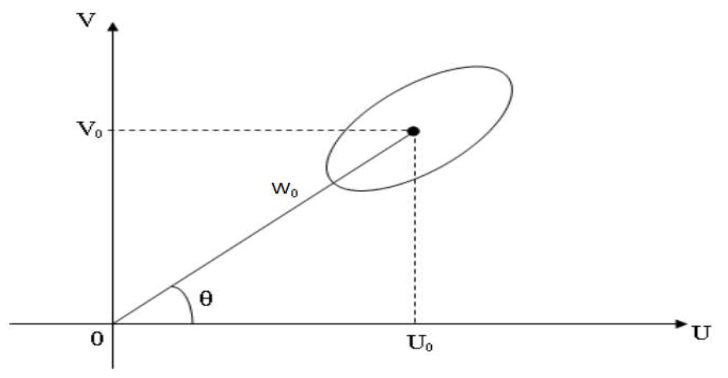
\includegraphics[width=0.65\textwidth]{Figures/gaborFig} % Include the image .png
	
	\caption{Contour à mi-niveau de la réponse en fréquence d’un filtre de Gabor 2D de fréquence centrale $W_0$ et d’orientation $\theta$.}
\end{figure}

L'utilisation des filtres de Gabor permet d'extraire de l'image considérée des informations pertinentes, à la fois en espace et en fréquence. Ils peuvent capturer le spectre de fréquence d'une image, en amplitude et en phase. Ces filtres sont toujours utilisés par bancs dans lesquels chacun des filtres est réglé à une orientation et une fréquence précise. Les recherches conduites dans la littérature montrent que les fonctions de Gabor simulent de manière convenable le système visuel humain en reconnaissance des textures; le système visuel étant considéré comme un ensemble de canaux de filtrage dans le domaine fréquentiel.
 \begin{figure}[H]
 	\label{fig:gabor49}
 	\centering
 	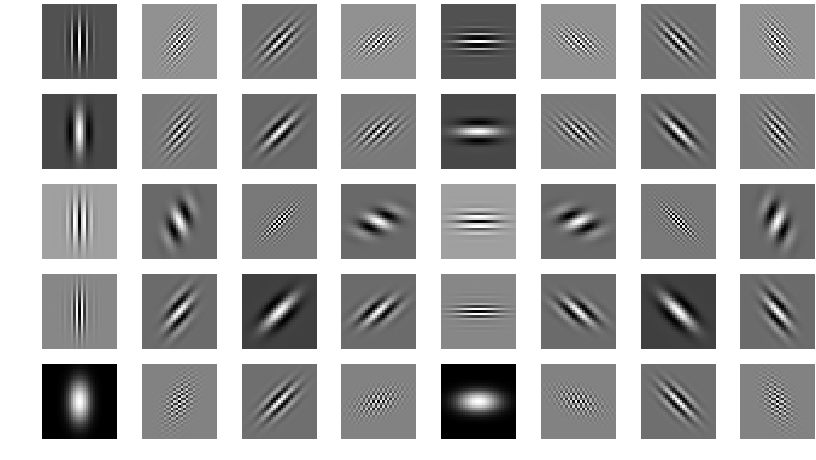
\includegraphics[width=0.65\textwidth]{Figures/gabor49} % Include the image .png
 	
 	\caption{Exemple du module des filtres de Gabor dans le domaine spatial.}
 	
 \end{figure}
 
 
%\subsubsection{Conclusion}
%
%Au même titre que l'information relative aux couleurs, Les attributs texturaux sont des attributs très importants pour la description de l'image et la reconnaissance de ses objets, cependant elles ne suffisent pas pour une bonne représentation du contenu de l'image, un inconvénient qui nécessite un autre attribut essentiel qui est celui de la forme.\\
%
%Dans la suite nous allons introduire cet attribut et les différentes approches utilisées pour
%l'extraire.

\subsection{Descripteur de forme}
Comme c'était le cas pour la texture, l'information de la forme est complémentaire de celle de la couleur pour la description de l'image.  Si l'être humain est particulièrement sensible à l'attribut de couleur pour distinguer les objets, pour certains types d'ambiguïté cela n'est pas suffisant et l'on a besoin de l'attribut de forme. La forme est généralement une description très riche d’un objet. Elle permet de détecter un objet sur une image plutôt que l’image elle-même. L’extraction d’attribut géométrique a été l’objet de la recherche d’images par le contenu ces dernières années.\\

La forme est un descripteur très important dans l'indexation des images. Elle est utilisée pour décrire la structure géométrique générique du contenu visuel. Généralement, les descripteurs de formes se divisent en deux catégories: 
\begin{itemize}
	\item les méthodes régions s'appuient sur la forme entière (règion). 
	\item les méthodes régions s'appuient sur le contour.
\end{itemize}
On peut ensuite distinguer deux familles pour chacune de ces catégories, une famille qui considère les objets comme une seule partie, et celle qui décrit les objets en les considérant comme un assemblage de sous parties. Une segmentation des objets est généralement utilisée avant l'extraction des attributs.\\

Les techniques d’extraction de forme par régions font référence aux moments invariants et sont utilisés pour caractériser l’intégralité de la forme d’une région. Ces attributs sont robustes aux transformations géométriques comme la translation, la rotation et le changement d’échelle [ElAsnaoui17]. La seconde approche fait classiquement référence aux descripteurs de Fourier et porte sur une caractérisation des contours de la forme. Ils ne peuvent pas détecter la structure interne de la forme puisqu’ils sont basés sur les contours uniquement. En outre, ces méthodes ne sont pas adaptées aux formes disjointes ou creuses, qui est le cas des symboles graphiques, car l’information sur le contour n’est pas disponible. Par conséquent, elles sont limitées à un certains types d’applications [Tabb06].

\begin{figure}[H]
	\label{fig:forme}
	\centering
	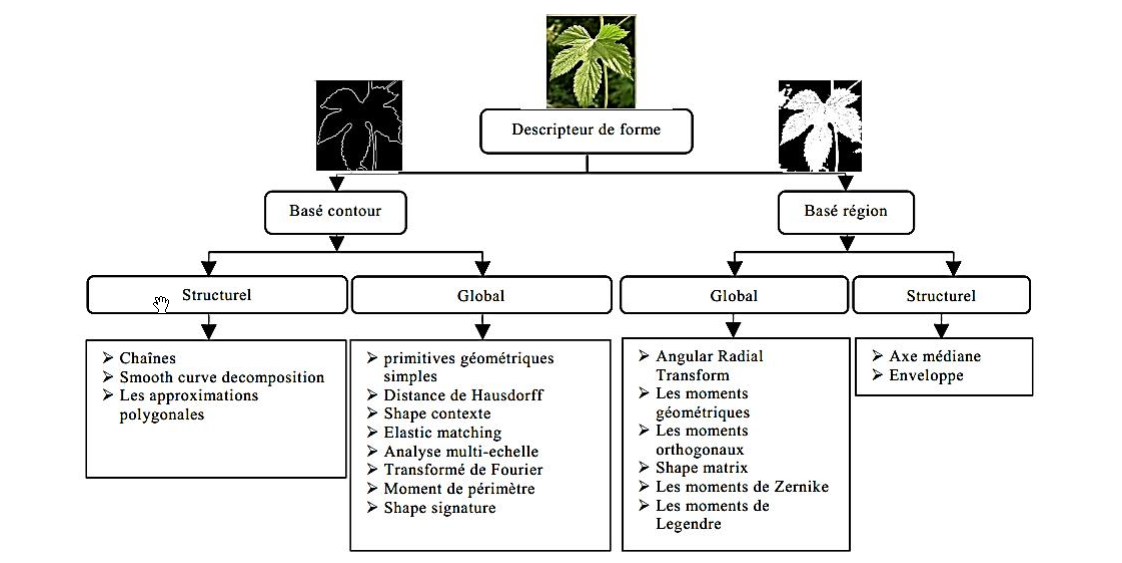
\includegraphics[width=1\textwidth]{Figures/forme} % Include the image .png
	
	\caption{Classification des méthodes d'extraction de forme.}
	
\end{figure}

Le problème fondamental est de déterminer si deux objets sont similaires, indépendamment de leur position dans l’image. C’est-à-dire l’invariance aux similitudes planes (Translation suivie d'une rotation et d’une homothétie). Il est bien connu que les descripteurs de forme invariants doivent satisfaire certains critères parmi lesquels : la robustesse vis à vis des faibles variations de formes et des approximations numériques, et la simplicité pour le calcul en « temps réel ».\\

Dans la suite nous présentons quelques-unes de ces méthodes.

\subsubsection{Descripteurs de Fourier}
Les descripteurs de Fourier (DFs) font partie des descripteurs les plus populaires pour les applications de reconnaissance de forme et de recherche d'images. Transformée de Fourier est une représentation fréquentielle d’une image, elle consiste de remplacer chaque région par des différentes fréquences spatiales. Les descripteurs de Fourier font partie des descripteurs basés sur les contours, ils ont souvent été utilisés par leur simplicité et leurs bonnes performances en terme de reconnaissance [Zhang05] et facilitent l'étape d’appariement. De plus, ils permettent de décrire la forme de l’objet à différents niveaux de détails.\\

Les DFs sont calculés à partir du contour des objets. Leur principe est de représenter le contour de l'objet par un signal 1D, puis de le décomposer en séries de Fourier. Les DFs sont généralement connus comme une famille de descripteurs car ils dépendent de la façon dont sont représentés les objets sous forme de signaux.

\subsubsection{Moments géométriques}
Les moments géométriques [Sonka99] permettent de décrire une forme à l’aide de propriétés
statistiques. Ils représentent les propriétés spatiales de la distribution des pixels dans l’image. La formule générale des moments géométriques est donnée par la relation suivante :

\begin{equation}
	M_{p,q} = \sum_{x=0}^{M-1}\sum_{y=0}^{N-1} x^p y^q f(x, y)
\end{equation}

avec $p+q$ est l'ordre du moment. Le moment d’ordre 0 $(M_{0,0})$  représente l’aire de la forme de l'objet, $f(x, y)$ : luminance du pixel $(x, y)$, c’est-à-dire noir ou blanc en binaire.

Les deux moments d'ordre $1 (M_{1,0})$ et $(M_{0,1})$, associés au moment d’ordre $0 (M_{0,0})$ permettent de calculer le centre de gravité de l'objet. Les coordonnées de ce
centre sont:

\begin{equation}
		\begin{tabular}{cc}
		$\bar{x} = \frac{M_{1,0}}{M_{0,0}}$ & $\bar{y} = \frac{M_{0,1}}{M_{0,0}}$
		\end{tabular}
\end{equation}
Il est possible de calculer à partir de ces moments l’ellipse équivalente à l’objet. Afin de calculer les axes de l’ellipse, il faut ramener les moments d’ordre 2 au centre de gravité :

\begin{equation}
\begin{tabular}{ccc}
$m_{2, 0}^g = M_{2,0} - M_{0,0} \bar{x}^2$ & $m_{1,1}^g = M_{1,1} - M_{0,0} \bar{x}\bar{y}$ 
& $m_{0,2}^g = M_{0,2} - M_{0,0} \bar{y}^2$ 
\end{tabular}
\end{equation}

Puis on détermine l’angle d’inclinaison de l’ellipse $\alpha$:
\begin{equation}
    \alpha = \frac{1}{2} \arctan(\frac{2m_{1,1}^g}{m_{2, 0}^g-m_{0,2}^g})
\end{equation}

Les moments géométriques sont très robustes et peu sensibles au bruit, préservation de l’information, facilement calculés et implémentés. Par contre, cette approche a des inconvénients comme la difficulté à corréler les moments avec la forme en elle-même, très sensible aux déformations et le temps de calcul de ces moments est très long.

\subsubsection{Les  moments de Hu}
À partir des moments géométriques, Hu [Hu62] a proposé en 1962 un ensemble de sept moments appelés moments de Hu. Ils sont invariants aux translations, rotation et changement d’échelle pour décrire une image. Par contre, ils sont très sensibles au bruit ce qui peut être un gros inconvénient dans un système de recherche d’images.\\

Nous les présenterons dans le chapitre 4.


\subsubsection{Moments orthogonaux}
Par opposition aux moments géométriques qui sont définis par rapport à une base quelconque $(x^p, y^q)$, les moments orthogonaux, comme leur nom l’indique, sont définis dans une base orthogonale, ce qui évite la redondance des informations portées par chacun des moments. Les deux types de moments orthogonaux les plus utilisés sont : les moments de Legendre et les moments de Zernike. (Les moments de Zernike a voir dans le chapitre 4) .

\subsubsection{Transformation ART}
Angular Radial Transform (ART) est un descripteur de forme robuste au changement d’échelle, à la translation et à la rotation et utilisé dans plusieurs travaux [Chawki16] et [AlAsnaoui17]. Ce descripteur consiste à projeter l’objet à étudier sur une série de fonctions de base [Kim99].

ART est un descripteur de formes par approche région qui caractérise la distribution des pixels dans un objet ou une région 2D. Il est basé sur l’étude des frontières et des pixels internes de la région à décrire. Il s’applique à un grand nombre d’objets, comme des objets complexes constitués de multiples régions discontinues ou des objets simples avec ou sans trou. Le descripteur de formes par approche régions se calcule en décomposant la forme sur plusieurs fonctions de base 2D orthogonales, définies par la transformation ART. Les coefficients ainsi obtenus sont utilisés après normalisation et quantification pour décrire la forme. ART donne un moyen compact et efficace pour exprimer la distribution de pixels dans une région de l’objet 2D [AlAsnaoui17]. Il peut décrire les deux formes de la région connectés et déconnectés.\\

L’ART [Kim99] décrit une forme à travers la distribution de ses pixels de façon invariante aux transformations affines. La transformation ART est utilisée comme descripteur par approche
région dans le standard MPEG-7. Elle est définie par la formule suivante :

\begin{equation}
    F_{nm} = {\int }_0^{2\pi} {\int }_0^{1} V_{nm}(\rho, \theta) f(\rho, \theta) \rho d\rho  d\theta
\end{equation}

Dans cette formule, $ F_{nm} $ est un coefficient d’ART d’ordre $ n $ et $ m $ , $ f(\rho, \theta) \longrightarrow {0,1} $ est une fonction image binaire définie en coordonnées polaires, et$  V_{nm}(\rho, \theta) $ st une fonction de base d’ART qui est séparable dans la direction angulaire et radiale :
\begin{equation}
	V_{nm}(\rho, \theta)= A_m(\theta) R_n(\rho) 
\end{equation}
où
\begin{equation}
\begin{tabular}{cc}
 $ A_m(\theta) =\frac{1}{2\pi}\exp(jm\theta) $ 
    & $ R_n(\rho) = \left\{
    \begin{array}{cc} 
    1 & n=0 \\ 2\cos( n \pi \rho) 
    & n \neq 0  \end{array} \right. $ 
\end{tabular}
\end{equation}

Le descripteur ART est alors défini comme l’ensemble des coefficients $ F_{nm} $ où $ m $ et $ n $ désignent les nombres de coefficients considérés.

 \begin{figure}[H]
	\label{fig:art}
	\centering
	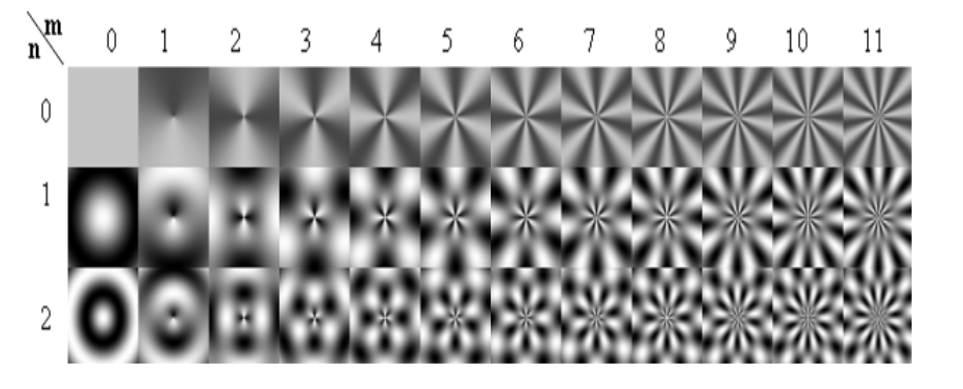
\includegraphics[width=0.65\textwidth]{Figures/art} % Include the image .png
	
	\caption{Parties réelles des fonctions de base d’ART.}
	
\end{figure}

La fonction de base d’ART $ V_{nm} $ est une fonction complexe. Sur la figure ci-dessus (Figure 2.10), les parties imaginaires sont identiques aux parties réelles, avec une différence de phase. La partie réelle de chaque fonction de base est présentée sous forme d’images.\\

Pour chaque image donnée, il y aura $ n \times m $  coefficients ART. Ces coefficients sont utilisés pour mettre en correspondance deux images. Le problème est de savoir combien de coefficient est nécessaire pour la description d’une image. Pour déterminer le nombre de coefficients, il faut analyser les covariances entre les fonctions de base. Par définition, le comité MPEG-7 [Jean01] maintient le nombre des valeurs de n plus petit que celui de m. Il propose de fixer n à 3 et m à 12. Ce sont les valeurs que nous utilisons dans notre étude.\\


Les méthodes d’indexation et de recherche doivent posséder les propriétés d’invariance aux
transformations géométriques subies par un objet à l’intérieur d’une image. ART présente certains avantages tels que :
\begin{itemize}
	\item  Robustesse aux changements d’échelle et aux translations.
	\item Invariance aux rotations.
	\item  Robustesse à la présence de bruit.
\end{itemize}

%\subsubsection{Conclusion}
%L'information relative à la forme est particulièrement importante dans la description d'une image. Plusieurs études ont été menées pour trouver un critère de choix des descripteurs de la forme pour l'indexation des images pour combler les manques des descripteurs couleur et texture.\\
%
%Pour rechercher des formes similaires, des mesures de similarité entre des descripteurs sont définies pour déterminer la distance entre eux. Cependant, la comparaison n’est pas toujours simple et elle exige parfois des transformations. De plus, la dimension du descripteur est souvent élevée, ce qui augmente la complexité quand on cherche des objets similaires dans une grande collection.\\
%
%Dans ce qui suit, nous présenterons quelques mesures de similarités utilisé en recherche d'images par contenu.

%
% Les descripteurs basés sur le contour incluent les descripteurs de Fourier [Rui 98], [Zhang 05], et les chaînes de Freeman, qui ont été largement utilisés.
% 
%  Les descripteurs basés sur la région prennent en compte tous les pixels de la forme et les méthodes les plus courantes sont basées, sur la théorie des moments [Prokop 92], [Hu 62], [Jiang 91], [Taubin 92].
%   
%   Les moments invariants offrent une description robuste aux transformations affines, propriété appréciable pour les systèmes CBIR.
%
%Quelle que soit la méthode utilisée, il demeure important que certaines propriétés d'invariance soient vérifiées, notamment pour la translation, le changement d’échelle et la rotation, du fait que l’être humain corrige instinctivement les effets de ces transformations lors de la recherche d’un objet. Dans certaines applications, la robustesse à l’occultation peut également être souhaitée.
%


\section{Les mesures de similarité entre attributs}
L'étape de la recherche dans les systèmes CBIR est la raison d'être d'un tel système et nécessite des techniques de comparaison entres attributs d'image (signatures). La mesure de similarité est alors une étape fondamentale dans la recherche d'images par le contenu. Elle compte sur la mesure de la ressemblance visuelle entre une image requête et les images de la base.\\

Les performances d'un CBIR dépendent largement de la mesure de similarité utilisée pour la comparaison des descripteurs des images.  de la recherche mais également de la représentation des caractéristiques.\\

La mesure de similarité quantifie la proximité des images dans l'espace des caractéristiques. Elle est souvent métrique, les images sont considérées ressemblantes si la distance est faible. La complexité de calcul d'une distance doit être raisonnable par ce que dans un système CBIR cette tâche s'exécute en temps réel ou pseudo réel. D'autres paramètres entrent en jeu telle la dimension de l'espace caractéristique, la taille de la base... La méthode naïve de recherche calcule la distance entre la requête et toutes les images de la base puis les ordonne selon leur score. Ceci par conséquent rend le temps de réponse proportionnel au nombre d'images $ (O(N)) $. Les méthodes d'indexation du contenu permettent par ailleurs de réduire cette complexité comparée à la recherche séquentielle (Exemple de M-Tree que nous présenterons dans le chapitre qui suit). 

Pour résumer, la mesure de similarité vérifie généralement les propriétés [Houari10]:

\begin{itemize}
	\item  \textbf{La perception} : Une faible distance dans l'espace de caractéristique indique deux images semblables.
	
	\item \textbf{Le calcul} : La mesure de distance se calcule rapidement pour une faible latence.
	
	\item \textbf{La scalabilité }: Le calcul de distance ne doit pas être affecté par une modification de taille de la base.
	
	\item \textbf{La robustesse} : La mesure devra être robuste aux changements des conditions d'acquisition d'image.
\end{itemize}

En mathématiques, on appelle distance sur un ensemble $E$ une application $d$ définie sur le produit $E^2 = E \times E$ et à valeurs dans l'ensemble $R^+$ des réels positifs:

\begin{equation}
	d: E \times E \rightarrow R^+
\end{equation}

vérifiant les propriétés suivantes :
\begin{table}[H]
	\caption{Les propriétés d'une distance.}
\begin{figure}[H]
	\centering
	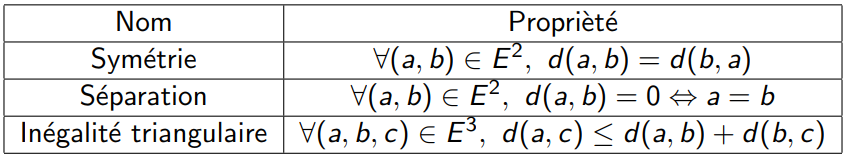
\includegraphics[width=0.8\textwidth]{Figures/distanceProp.png} % Include the image .png
\end{figure}
\end{table}

Un ensemble muni d'une distance est un espace métrique.\\

Au lieu d'un appariement exact, la recherche d’images par le contenu calcule des similarités visuelles entre une image requête et les images de la base d'images. En conséquent, le résultat d'une recherche n'est pas une seule image mais une liste d'images ordonnées selon leur degré de similitude avec l'image requête. Plusieurs mesures de similarités ont été proposées dans la littérature. Les différentes mesures de similarité influencent les performances de recherche des systèmes de recherche par le contenu.\\

Le choix de la mesure de similarité la plus appropriée dépend du niveau d'abstraction de la
représentation de l'image : images brutes (pixels) ou attributs (vecteurs descripteurs).
\begin{itemize}
	\item \textbf{Images brutes (pixels): }Au plus bas niveau d'abstraction, les images sont tout simplement des agrégations de pixels. La comparaison entre les images, est réalisée pixel par pixel, et les mesures de similarité couramment utilisées comprennent : le coefficient de corrélation, la somme des valeurs absolue des différences (SVAD), la distance des moindres carrés, et l’information mutuelle.
	La comparaison au niveau des pixels est très spécifique et, par conséquent, n'est utilisée que lorsque des appariements relativement précis sont nécessaires.
	
	\item \textbf{Attributs:} Les attributs ou vecteurs descripteurs sont des valeurs numériques de données extraites des images ou des objets dans les images, tels que la couleur, la forme et la texture. Plusieurs mesures de similarité sont couramment utilisées pour la comparaison d’attributs: la distance euclidienne, la distance de Minkowsky et la distance d’intersection  [Khouloud09].
\end{itemize}

Julien Fauqueur à classifier les distances pour les distributions de couleurs [Fauqueurs03] comme suite:
\begin{table}[H]
	\centering
	\caption{Les classe de distances.}
	\begin{tabular}{|l|l|l|}
		\hline
		\textbf{\makecell{Distances cellule-à-cellule ou “daltoniennes”}
} & \textbf{Distances inter-cellules}\\
		\hline
		\makecell{- Les distances de Minkowski\\
		- Intersection d’histogrammes\\
	    - Test du $ \chi^2 $  \\
        - Divergence de Kullback Leibler\\
        - “Jensen Difference Divergence”} 
		& \makecell{- Histogramme cumulé\\
			- Histogramme flou \\ 
			- Distance Quadratique\\
			- Earth Mover Distance\\
			- “Weighted Correlation”
		 }   \\
		\hline 
	\end{tabular}
	
\end{table}

Ci-après les distances les plus utilisées pour comparer des images considérées comme vecteurs ou comme distributions statistiques. 

\subsection{Distances de Minkowski}
La distance de Minkowski est une famille de distances vectorielles. Soit $I_1$ , $I_2$ deux vecteurs de caractéristiques, elle s'exprime par :

\begin{equation}
        d_p(I_1, I_2) =  \sqrt[p]{\sum_{i=1}^{N} \left|{I}_{1}(i)-{I}_{2}(i)\right|^p} 
\end{equation}

Où $p\geq 1$ est le facteur de Minkowski et $N$ la dimension de l’espace caractéristique. Les métriques de Minkowski sont simples d’utilisation, rapides à calculer, simples à implémenter, et représentent un bon compromis entre efficacité et performance, par contre leur calcul est réalisé en considérant que chaque composante du vecteur apporte la même contribution à la distance. Pour cette famille de distances, plus le paramètre $p$ augmente, plus la distance $d_p$ aura tendance à favoriser les grandes différences entre coordonnées.

On distingue:
\begin{table}[H]
	\caption{Les distances de Minkowski}
	\begin{tabular}{|c|c|c|}
		\hline
		\textbf{Distance} & \textbf{Caractéristiques}\\
		\hline
		\makecell{Manhatttan : \\ $  d_1(I_1, I_2) = \sum_{i=1}^{N} \left|{I}_{1}(i)-{I}_{2}(i)\right|  $ } 
		& \makecell{Cette distance est plus convenable pour mesurer\\
			  la similarité entre les données  multivariées,\\ 
			 elle est moins sensible au  bruit\\
			 coloré que la distance euclidienne. }   \\
		\hline
		
		
		\makecell{Euclidienne :\\ $ d_2(I_1, I_2) =  \sqrt{\sum_{i=1}^{N} \left|{I}_{1}(i)-{I}_{2}(i)\right|^2} $}  
		& \makecell{C’est la distance la plus fréquemment \\
			utilisée grâce à ses propriétés géométriques \\
			intéressantes. Cette distance à tendance à \\
			donner plus d’importance aux plus grandes \\
			différences sur une variable simple. Le contour\\
			 de la même distance (Euclidienne) à partir d’un \\
			 point donnée à  une forme sphérique \\(cercle en deux dimensions).}   \\
		\hline
		
		\makecell{Chebychev :\\ 
			$d_{\infty}(I_1, I_2)=\max_{i=1}^N \left|{I}_{1}(i)-{I}_{2}(i)\right|$  
		} 
		 & \makecell{La distance de Chebychev est adaptée \\
		 	aux données de grande dimension, elle est \\
		 	souvent employée dans les applications où la\\
		 	 vitesse d’exécution est importante.\\ 
		 	 Cette distance examine la différence absolue\\
		 	  entre les différents pairs des vecteurs, elle\\
		 	   est considérée comme une approximation\\ 
		 	   de la distance Euclidienne mais\\
		 	    avec moins de calcul.} \\   
		\hline
		
	
	\end{tabular}
	
\end{table}

\subsection{Distance quadratique}
La distance de Minkowski traite les éléments du vecteur de caractéristique d’une manière équitable. La distance quadratique en revanche favorise les éléments les plus ressemblants. Les propriétés de cette distance la rendraient proche de la perception humaine de la couleur, ce qui en fait une métrique attractive pour les systèmes de Recherche d’images couleur par le contenu. Proposée dans [Hafner95], la distance couleur quadratique compare toutes les valeurs
de cellules des deux histogrammes qu’elle pondère par leur similarité couleur, Sa formule générale est donnée par :

	\begin{equation}
	d_q(I_1, I_2) = \sqrt{(I_1 - I_2)^T A (I_1 - I_2)} 
	\end{equation}



Ou $A = (a_{ij}) $est la matrice de similarité. $a_{ij}$ représente la distance entre deux éléments des vecteurs $I_1$ et $I_2$, elle est définie par :


\begin{equation}
	a_{ij} = 1 - \frac{d_{ij}}{ d_{max}} 
\end{equation}

Où $ d_{ij} $ est la distance dans l’espace couleur considéré et $ d_{max} $ le maximum global
de cette distance. Notons que si l’on remplace $  A $ par la matrice identité, nous retrouvons la distance euclidienne.
\subsection{Distance de Swain}
Cette mesure est l'une des premières distances utilisée dans la recherche d'image par le contenu, si les images d’une base des images sont indexées par des histogrammes, les distances géométriques s’appliquent. Cependant, il est possible de définir des mesures de similarité propres à cette représentation. Ainsi, l’intersection d’histogrammes est l’une des premières distances utilisée dans les systèmes CBIR [Swain91]. Elle permet de comparer deux histogrammes normalisés $H_1$ et $H_2$ . La distance de Swain s’exprime ainsi :

	\begin{equation}
	 d_2(H_1, H_2) = 1- \frac{\sum_{i=1}^{N} \min(H_1(i),  H_2(i))}{\sum_{i=1}^{N}  H_2(i)}  
	\end{equation}

\subsection{Distance de Canberra}
Elle est introduite par G. N. Lance et W. T. Williams [Lance67]. C'est une version
pondérée de la distance Manhattan. La distance de Canberra entre les vecteurs et dans un espace vectoriel réel à N dimensions est la suivante:

\begin{equation}
	d_c(I_1, I_2) = 1- \sum_{i=1}^{N}   \frac{\left|{I}_{1}(i)-{I}_{2}(i)\right|}{\left|{I}_{1}(i)\right| + \left|{I}_{2}(i)\right|}
\end{equation}


Il existe d’autres distances dans la littérature qui ne sont pas abordées dans ce mémoire.


\subsection{Conclusion}
Le choix des descripteurs ou mesures de similarité pour un système de recherche d'images par contenu est important, dans le sens où, ce choix influe sur les résultats attendus. Cependant, d'une part il n'y a pas d'attributs universels, et d'autre part le choix des descripteurs dépend fortement de la base d'image à utiliser et des connaissances à priori qu'on peut avoir sur la base.\\

Ce chapitre a fait l’état de l’art sans exhaustivité des différents descripteurs des attributs visuels pouvant être utilisés pour la recherche d’images par le contenu ainsi que les approches correspondantes. Aussi, nous avons dressé une liste des types de descripteurs et les mesures de similarités avec leurs avantages et leurs inconvénients. Le chapitre suivant se focalisera sur les méthodes d'indexation pour accélérer la recherche et leurs importance dans un systeme CBIR.